\thispagestyle{doisongtoanhocnone}
\pagestyle{doisongtoanhoc}
\everymath{\color{doisongtoanhoc}}
\graphicspath{{../doisongtoanhoc/pic/}}
\blfootnote{$^1$\color{doisongtoanhoc}Trung tâm Thông tin -- Tư liệu, Viện Hàn lâm Khoa học và Công nghệ Việt Nam.}
\begingroup
\AddToShipoutPicture*{\put(0,616){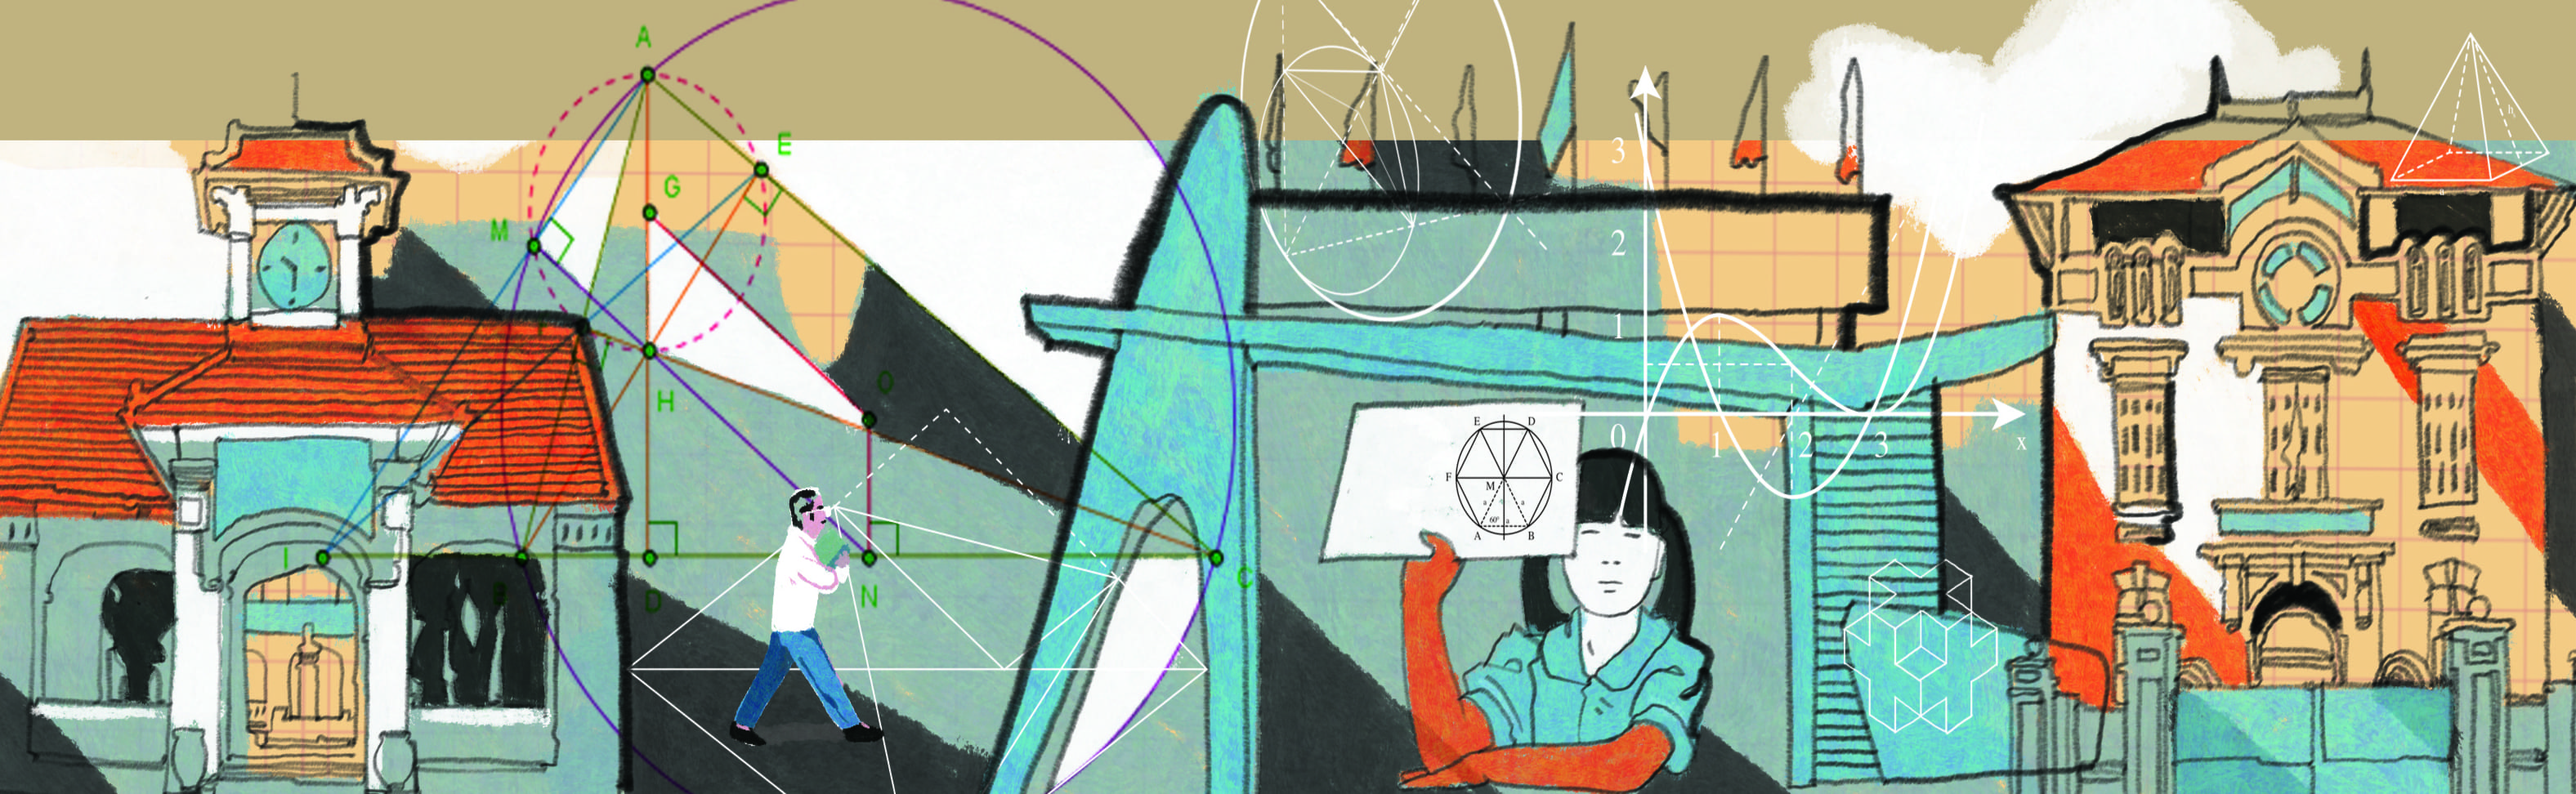
\includegraphics[width=19.3cm]{../bannerdoisong}}}
\AddToShipoutPicture*{\put(80,475){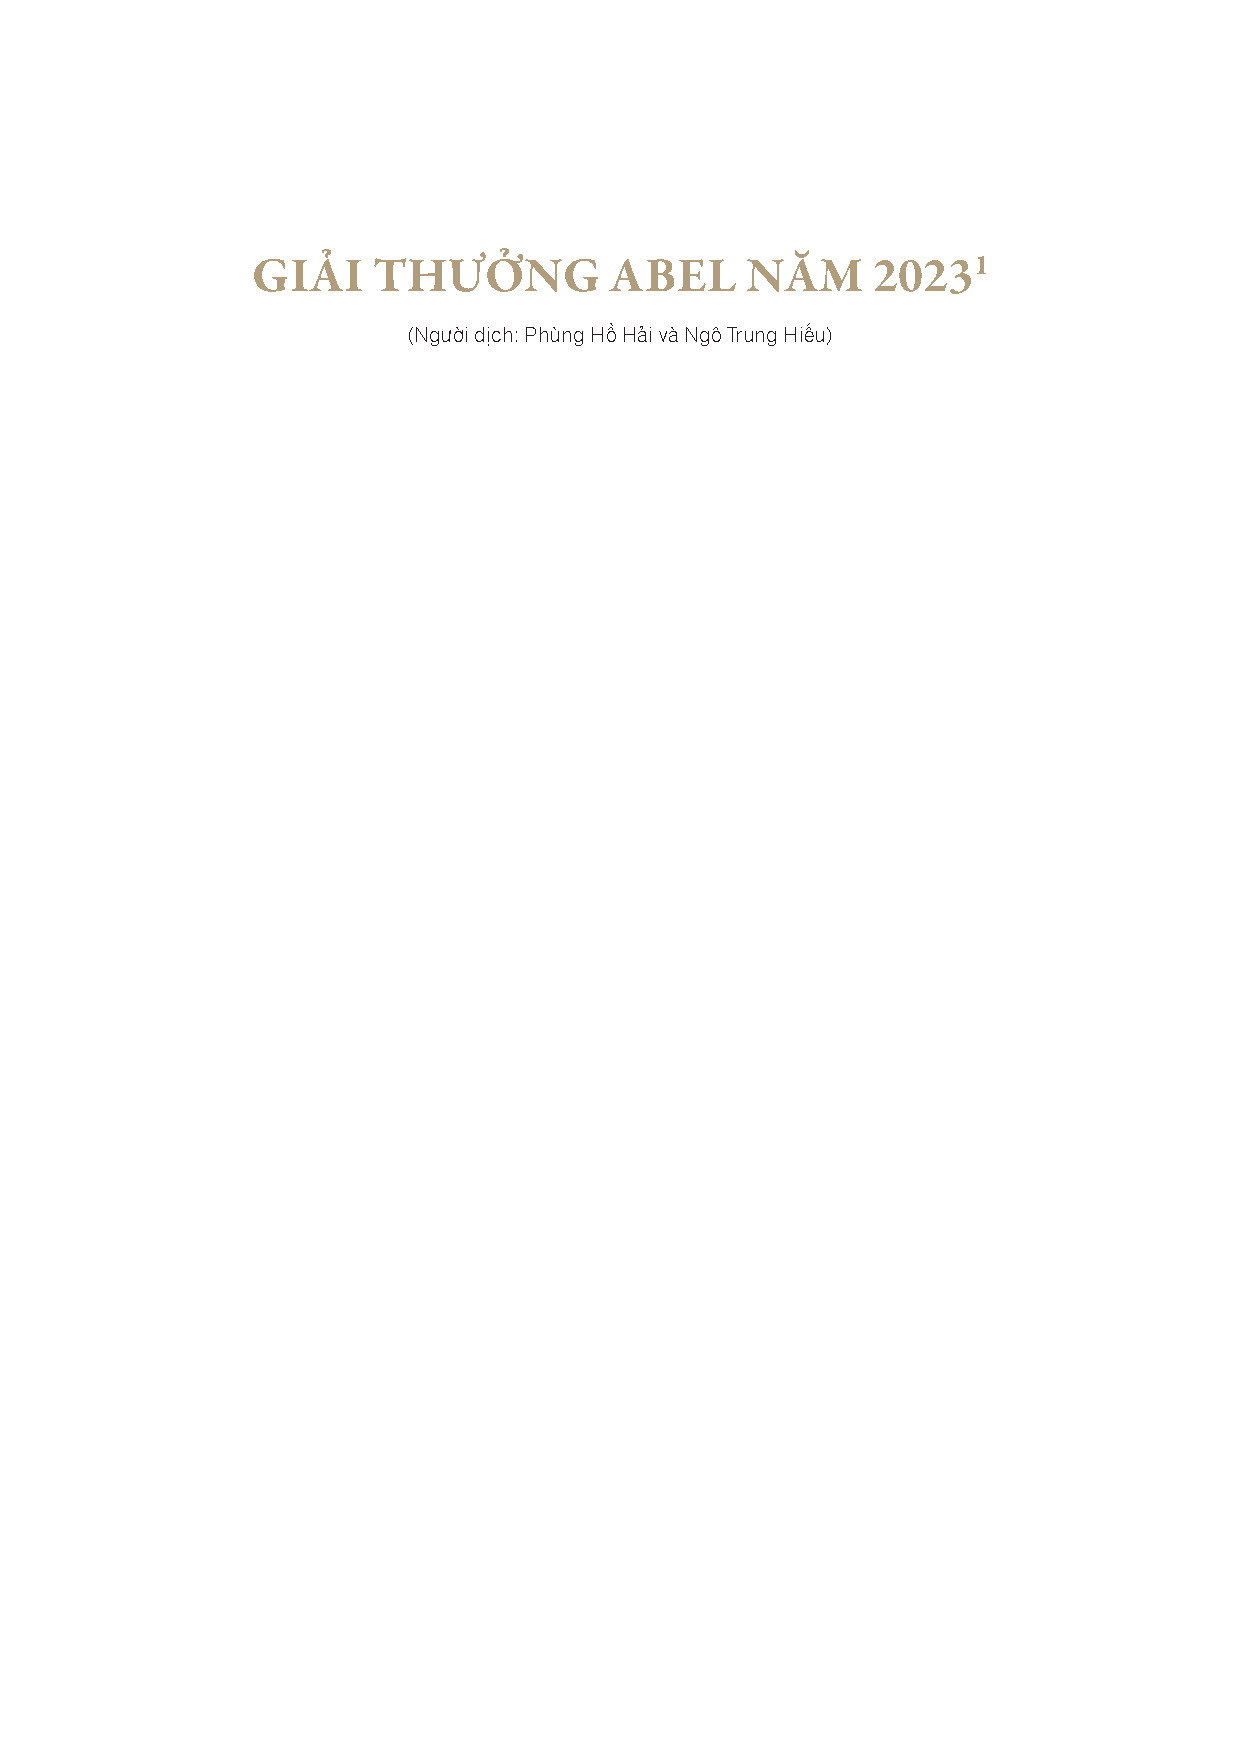
\includegraphics[scale=0.95]{../tieude.pdf}}}\centering
\endgroup

\vspace*{230pt}


\begin{multicols}{2}	
	Ngày $25/3/2023$, tại Hà Nội, Viện Toán học, Trung tâm Thông tin -- Tư liệu, Viện Hàn lâm Khoa học và Công nghệ Việt Nam và Trung tâm Quốc tế Đào tạo và Nghiên cứu Toán học (trực thuộc Viện Toán học, được UNESCO bảo trợ) đã đồng tổ chức ngày ``Toán học dành cho mọi người". Đây là hoạt động hưởng ứng Ngày Toán học Thế giới năm $2023$, đã thu hút đông đảo các nhà khoa học, giáo viên, sinh viên và học sinh trên cả nước tham dự.
	\vskip 0.1cm
	GS. Hoàng Tụy ($1927 - 2019$) là một nhà Toán học xuất sắc, đồng thời cũng là một nhà sư phạm mẫu mực. Trước khi biên soạn những giáo trình đại học được nhiều thế hệ sinh viên, nghiên cứu sinh sử dụng, GS. Hoàng Tụy từng biên soạn những bài giảng đầu tiên cho hệ thống giáo dục quốc dân. Cả cuộc đời cống hiến cho Toán học, Ông không ngừng trăn trở về nền giáo dục nước nhà. Được sự đồng ý của gia đình GS. Hoàng Tụy, Kỳ thi ``Bài giảng và bài viết về Toán học, mang tên Hoàng Tụy" được tổ chức với sự phối hợp của Tạp chí Pi và Trung tâm Quốc tế Đào tạo và Nghiên cứu Toán học.
	\vskip 0.1cm
	Với mục tiêu khích lệ sự tìm tòi, sáng tạo của giáo viên, sinh viên và mọi người yêu Toán học trong việc giảng dạy, đồng thời quảng bá Toán học, khơi dậy lòng say mê Toán học trong học sinh và công chúng, Kỳ thi ``Bài giảng và bài viết mang tên Hoàng Tụy" đã thu hút nhiều tác giả gửi hồ sơ tham gia. 
	\vskip 0.1cm
	Chủ đề của Kỳ thi lần thứ hai, năm $2023$ là: Tìm hiểu về môn Toán trong 	``Chương trình giáo dục phổ thông mới" thông qua một chủ đề cụ thể; Tìm hiểu về Toán sơ cấp, Lịch sử Toán học và Toán học trong cuộc sống. Hội đồng giám khảo năm nay gồm: 
	\vskip 0.1cm
	--	GS.TSKH. Ngô Việt Trung (Chủ tịch Hội Toán học Việt Nam, Nguyên Viện trưởng Viện Toán học), Chủ tịch Hội đồng;
	\vskip 0.1cm 
	--	GS.TSKH. Đỗ Đức Thái (Đại học Sư phạm Hà Nội, Phó Chủ tịch Hội Toán học Việt Nam);
	\vskip 0.1cm
	--	GS.TSKH. Phùng Hồ Hải (Phó Chủ tịch Hội Toán học Việt Nam, Nguyên Viện trưởng Viện Toán học);
	\vskip 0.1cm
	--	GS.TSKH. Hà Huy Khoái (Viện trưởng viện Toán học và khoa học ứng dụng Trường Đại học Thăng Long, Nguyên Viện trưởng Viện Toán học);
	\vskip 0.1cm
	--	TS. Trần Nam Dũng (Phó Hiệu trưởng Trường Phổ thông Năng khiếu, Đại học Quốc gia Thành phố Hồ Chí Minh);
	\vskip 0.1cm
	--	PGS. TS Phó Đức Tài (Trưởng khoa Toán--Cơ--Tin học, Trường Đại học Khoa học Tự Nhiên, Đại học Quốc gia Hà Nội).
	\begin{figure}[H]
		\vspace*{-5pt}
		\centering
		\captionsetup{labelformat= empty, justification=centering}
		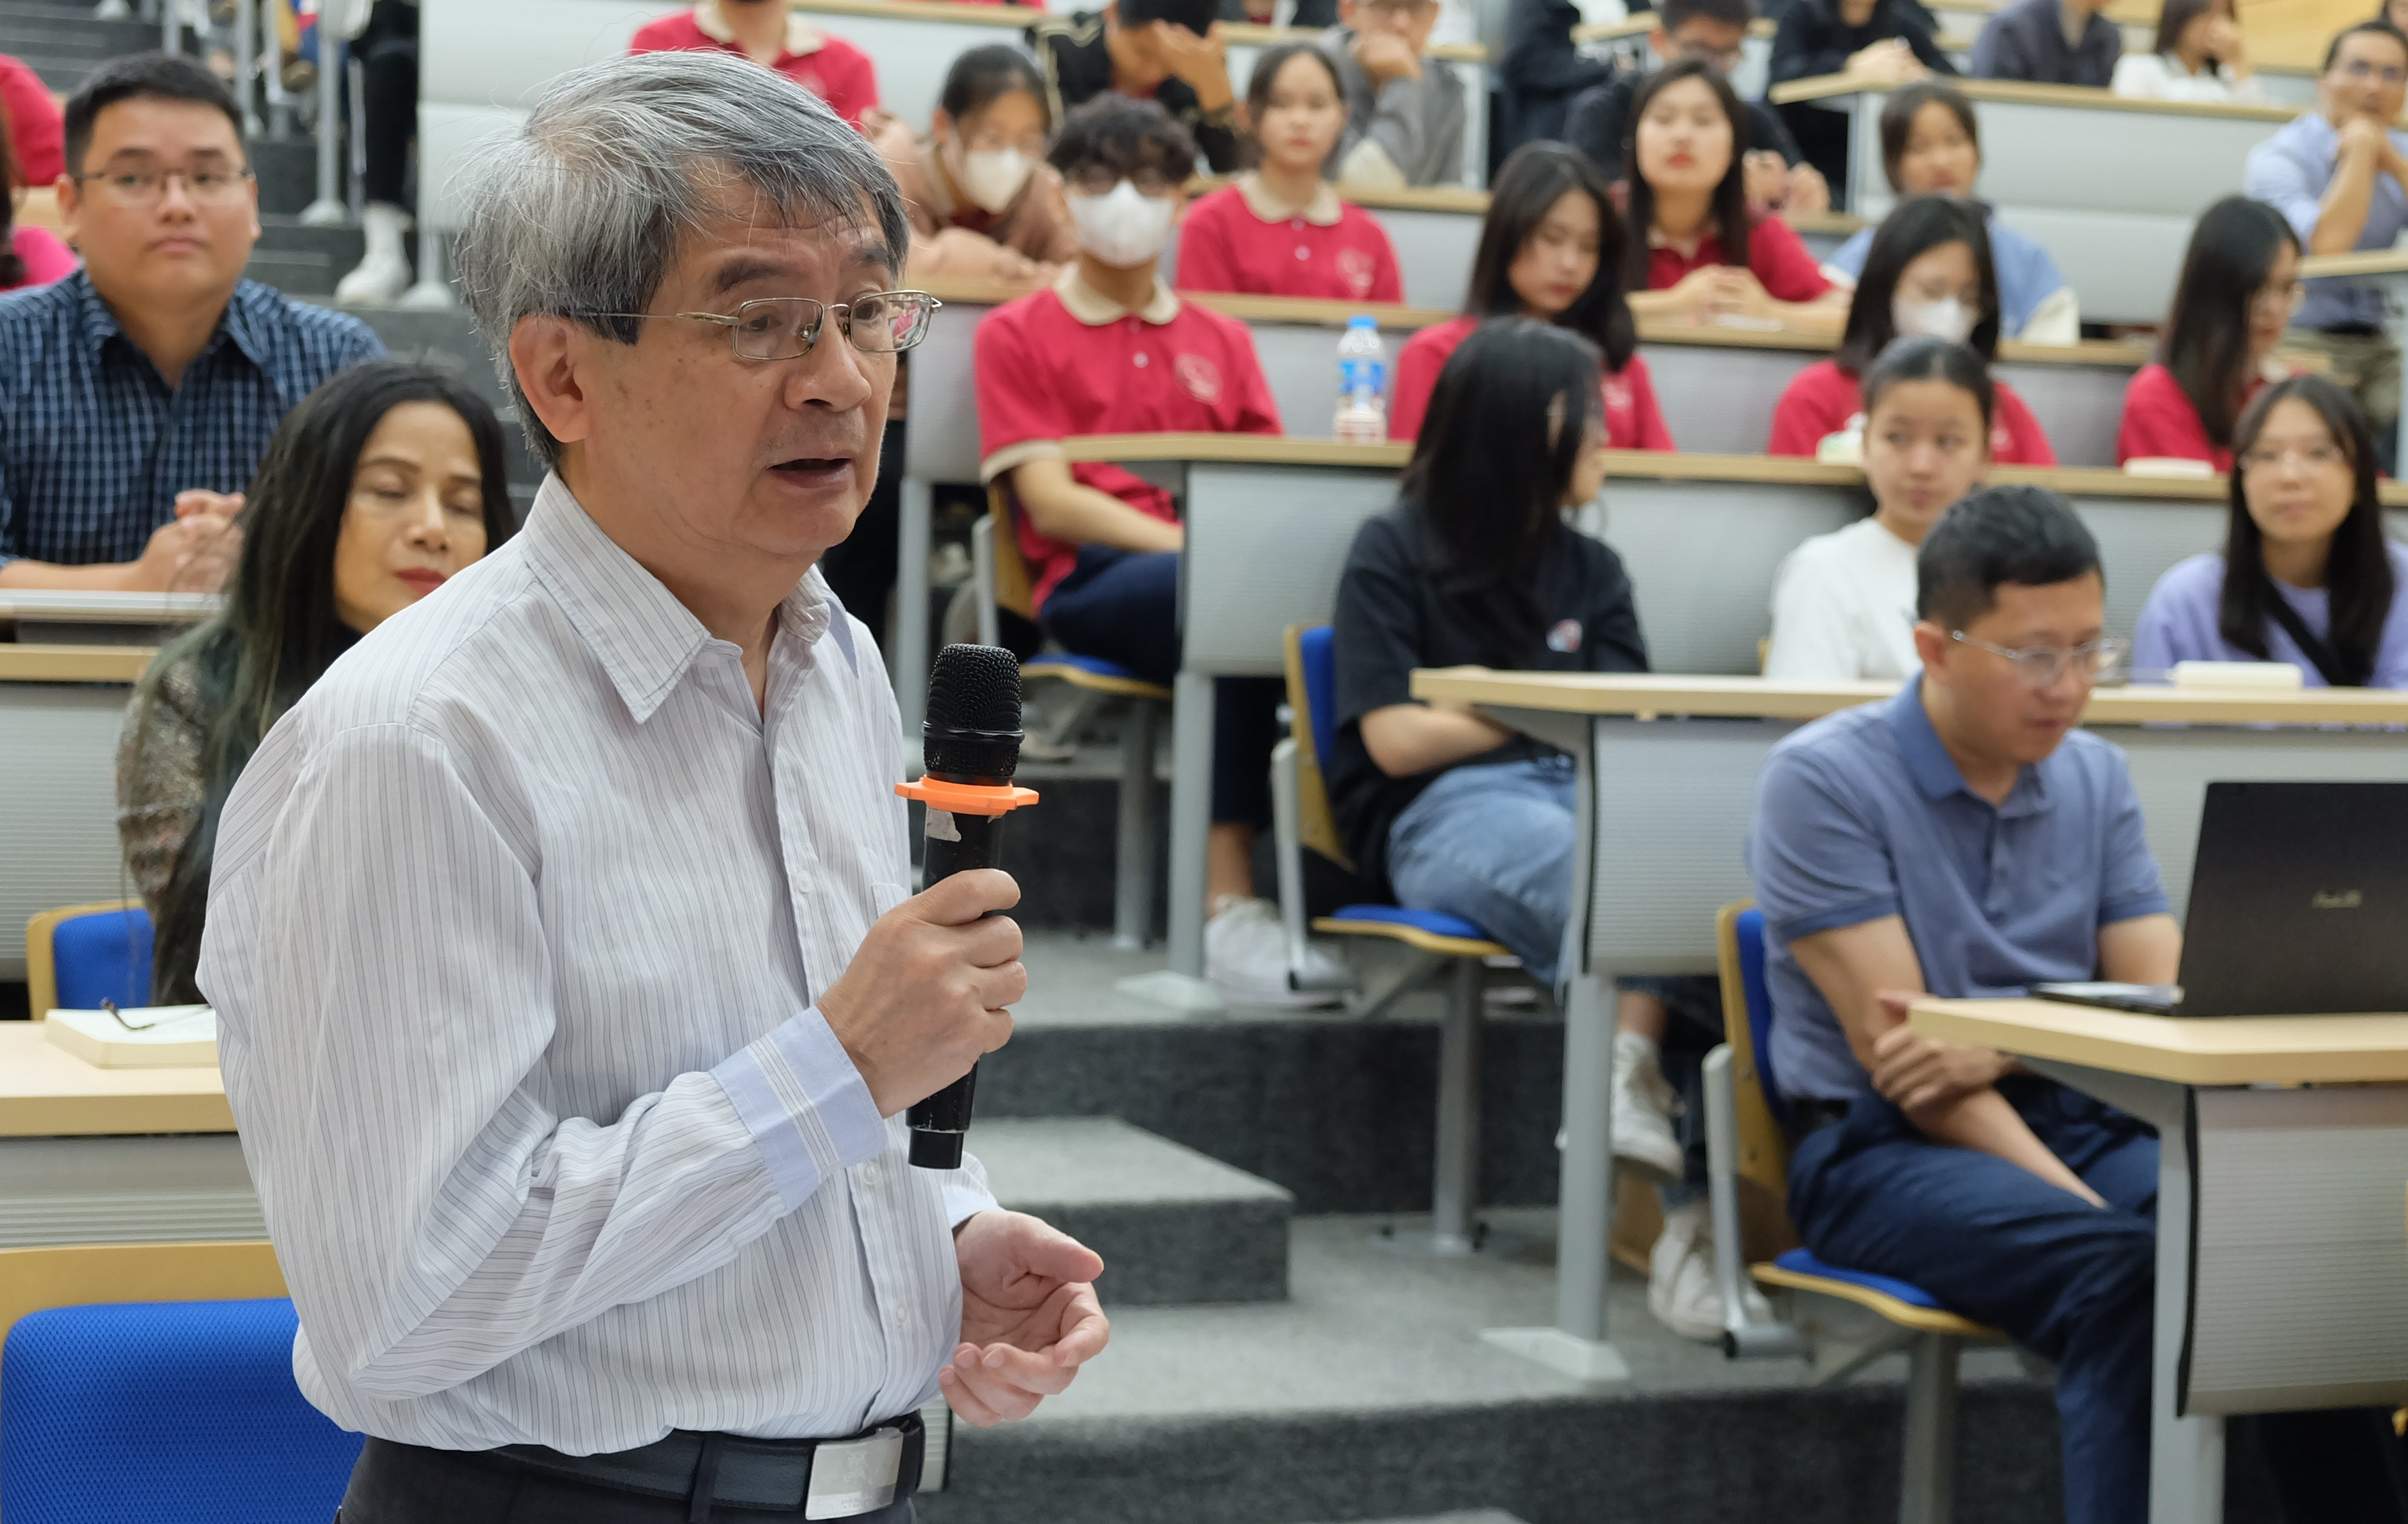
\includegraphics[width= 1\linewidth]{1}
		\caption{\small\textit{\color{doisongtoanhoc}Giáo sư Ngô Việt Trung, Chủ tịch Hội Toán học Việt Nam, Chủ tịch Hội đồng Giám khảo.}}
		\vspace*{-10pt}
	\end{figure}
	Ban Tổ chức đã tiến hành chấm các hồ sơ dự thi ở vòng sơ khảo, lựa chọn được $8$ hồ sơ tốt nhất để tranh tài tại vòng chung khảo, bao gồm: 
	\vskip 0.1cm
	$1$. Hình có trục đối xứng, tác giả Nguyễn Thụy Việt Anh, Trường Liên cấp Hội nhập Quốc tế Ischool, Quảng Trị; 
	\begin{figure}[H]
		\vspace*{-5pt}
		\centering
		\captionsetup{labelformat= empty, justification=centering}
		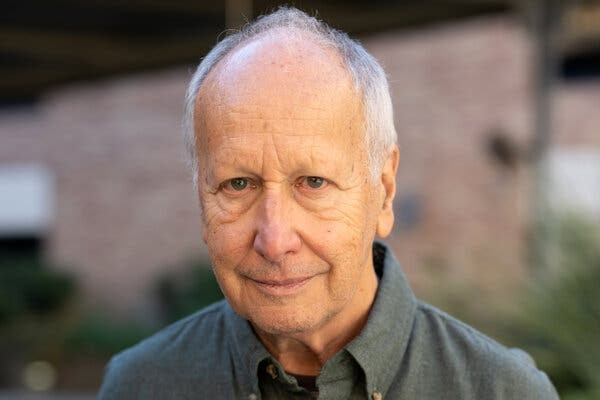
\includegraphics[width= 1\linewidth]{2}
%		\caption{\small\textit{\color{}}}
		\vspace*{-10pt}
	\end{figure}
	$2$. Lý thuyết đồ thị và các cấu trúc đáng chú ý, tác giả Hà Trung, Trường THPT chuyên Lê Hồng Phong, Nam Định; 
	\begin{figure}[H]
		\vspace*{5pt}
		\centering
		\captionsetup{labelformat= empty, justification=centering}
		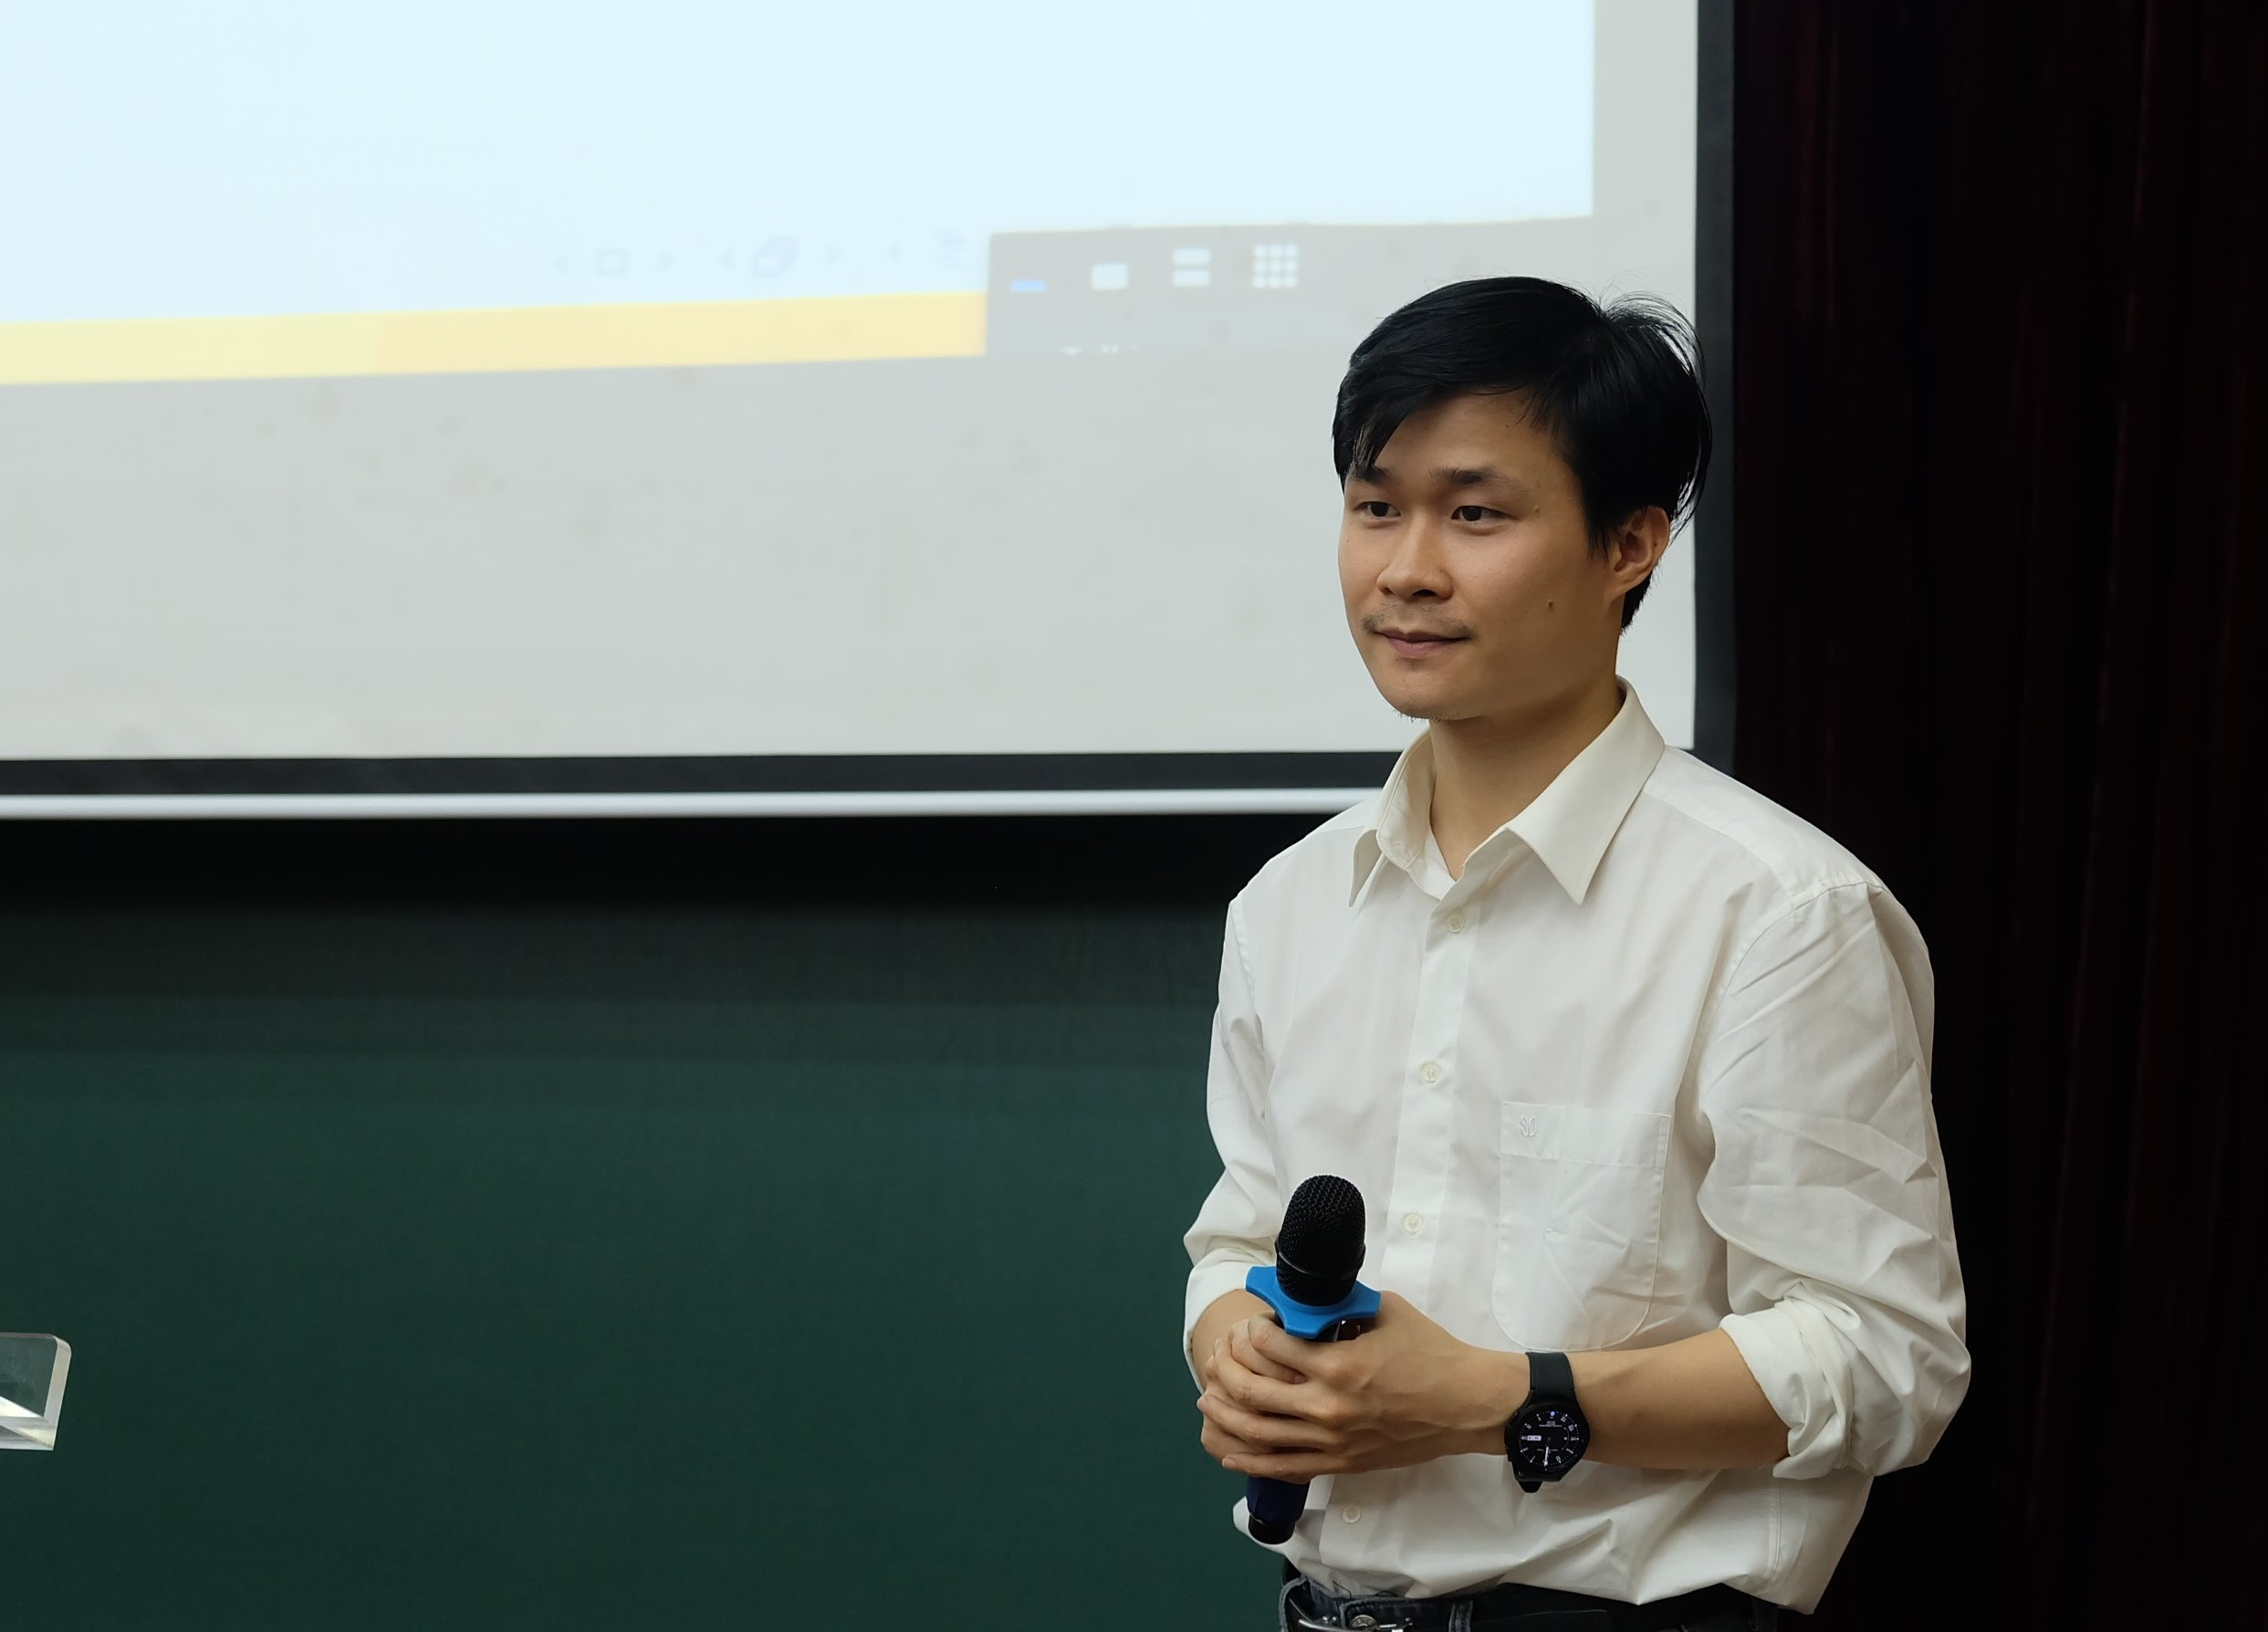
\includegraphics[width= 1\linewidth]{3}
%		\caption{\small\textit{\color{}}}
		\vspace*{-15pt}
	\end{figure}
	$3$. Bổ đề hai đoạn thẳng và một số ứng dụng, tác giả Nguyễn Hữu Tâm, Trường THPT chuyên Lê Quý Đôn, Bình Định; 
	\begin{figure}[H]
		\vspace*{-5pt}
		\centering
		\captionsetup{labelformat= empty, justification=centering}
		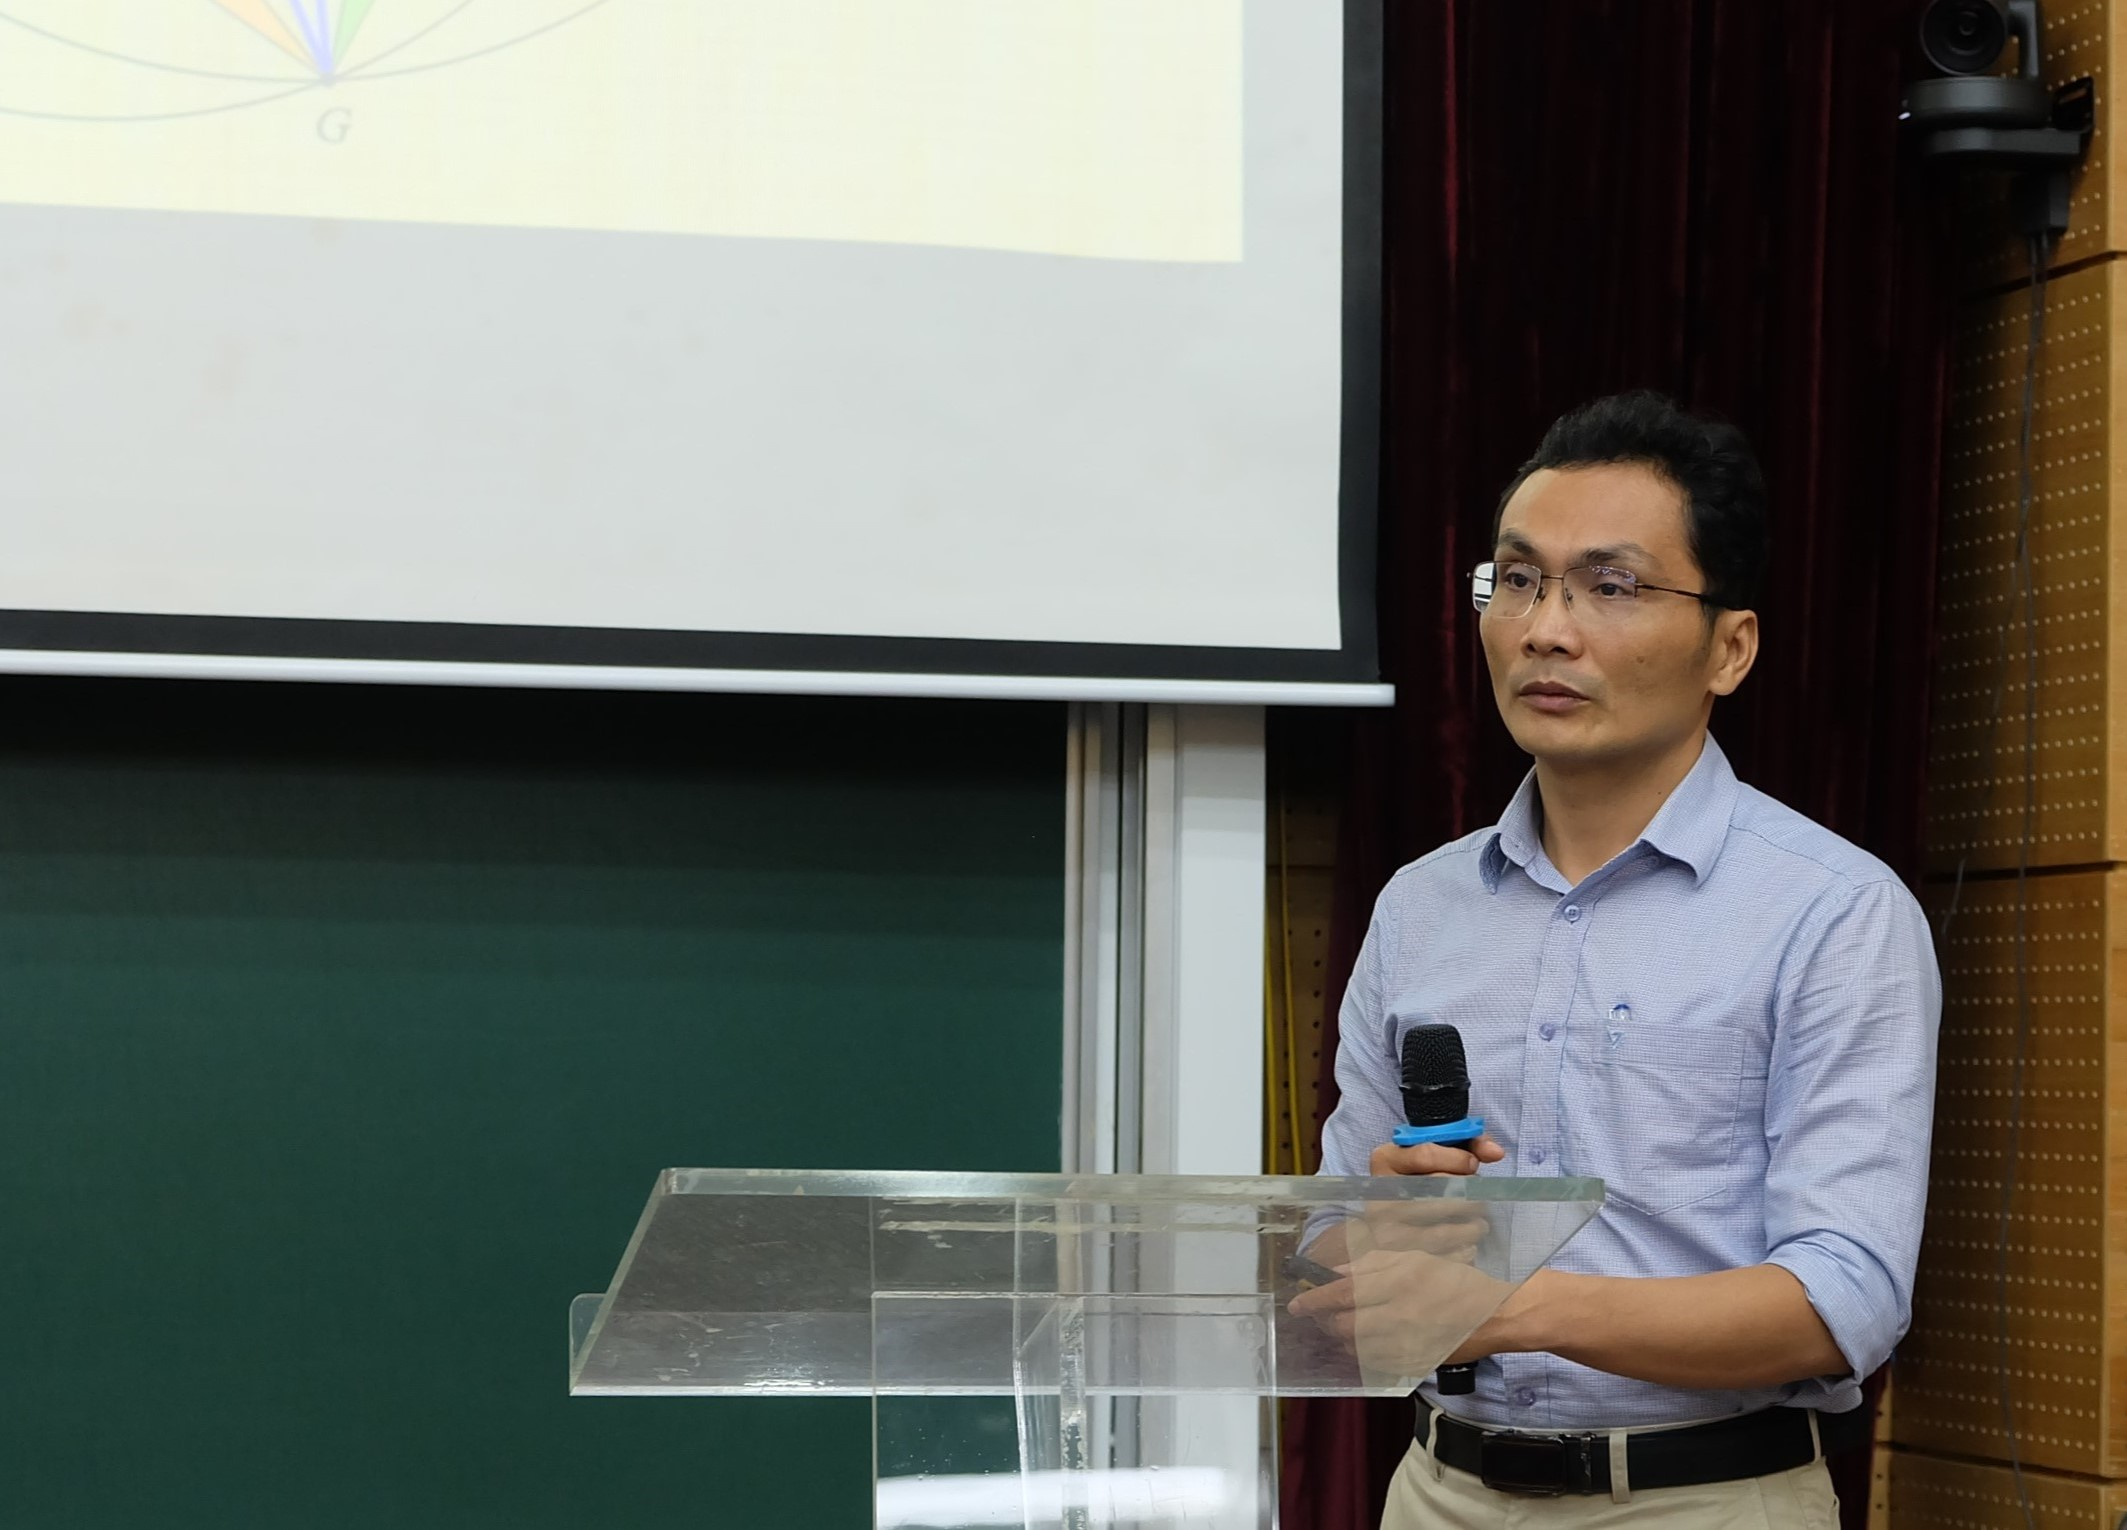
\includegraphics[width= 1\linewidth]{4}
%		\caption{\small\textit{\color{}}}
		\vspace*{-15pt}
	\end{figure}
	$4$. Nét đẹp của phương pháp đếm dưới góc nhìn của số Fibonacci, tác giả Nguyễn Tuấn Anh, Trường PTTH chuyên Nguyễn Quang Diêu, Đồng Tháp; 
	\begin{figure}[H]
		\vspace*{-5pt}
		\centering
		\captionsetup{labelformat= empty, justification=centering}
		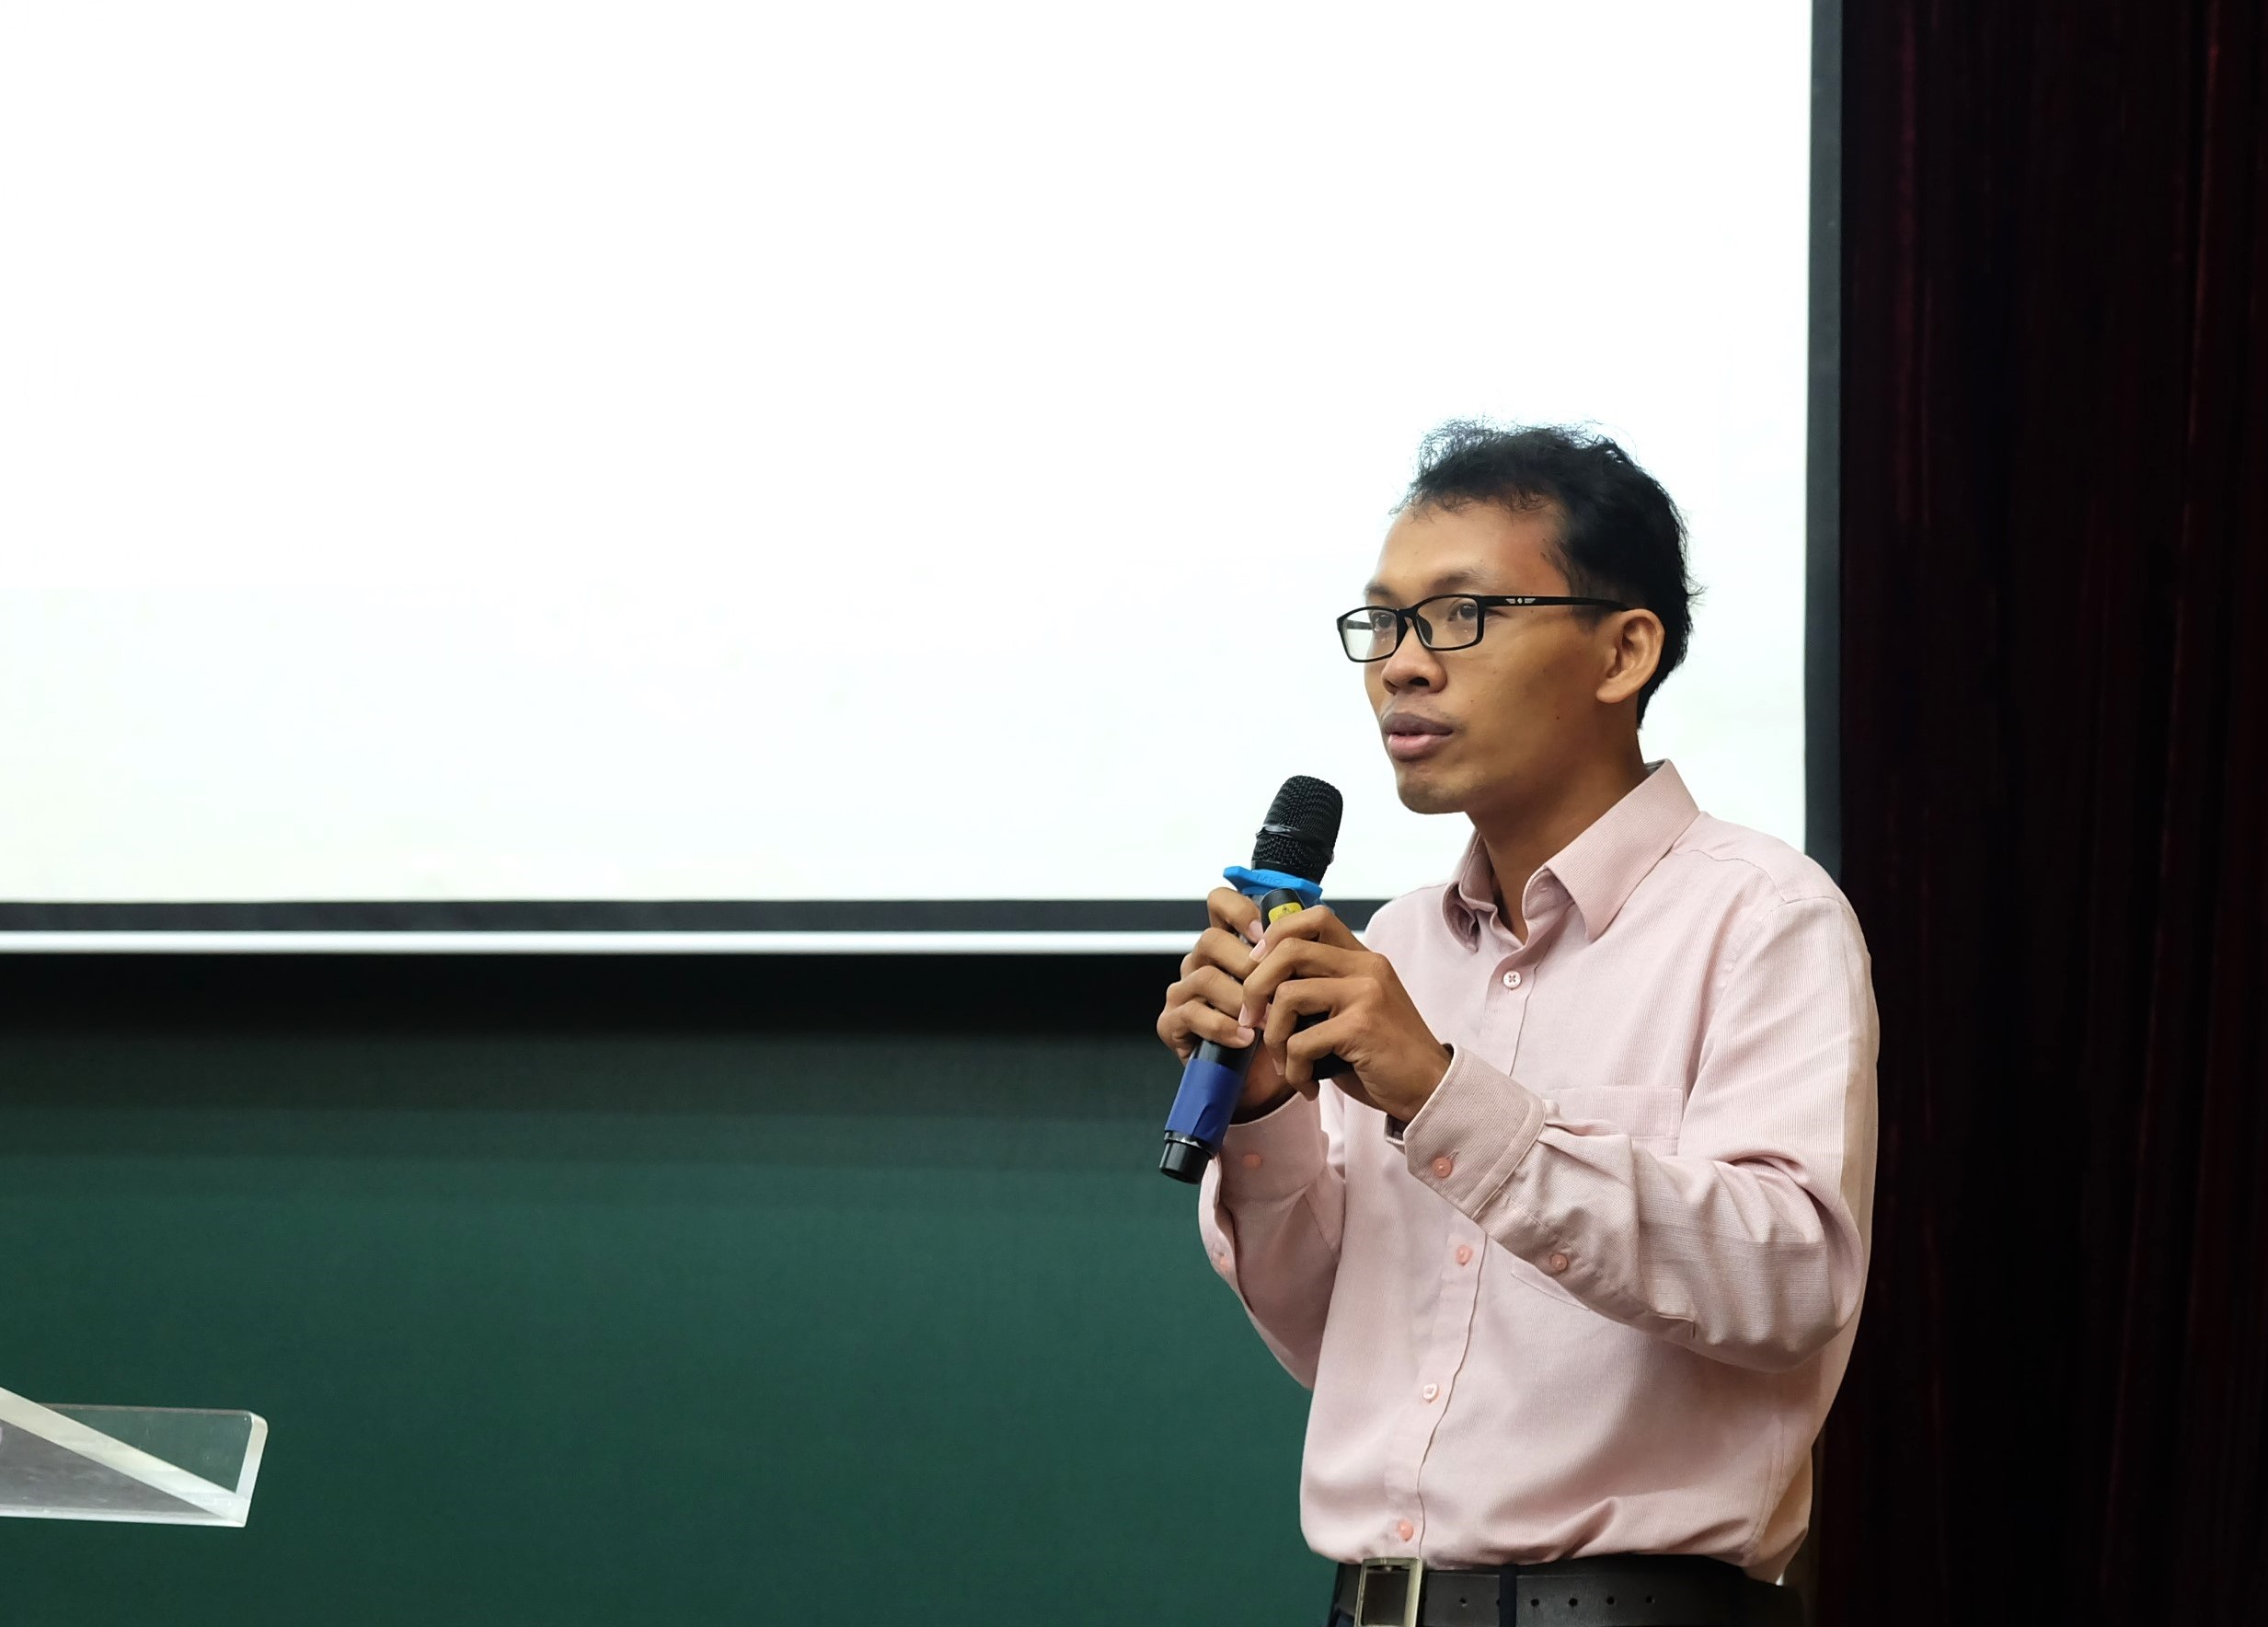
\includegraphics[width= 1\linewidth]{5}
%		\caption{\small\textit{\color{}}}
		\vspace*{-15pt}
	\end{figure}
	$5$. Một cách thiết kế dạy học Toán theo hướng gắn liền với thực tiễn, tác giả Phạm Đức Quang, Trường Đại học Hà Nội $2$; 
	\begin{figure}[H]
		\vspace*{5pt}
		\centering
		\captionsetup{labelformat= empty, justification=centering}
		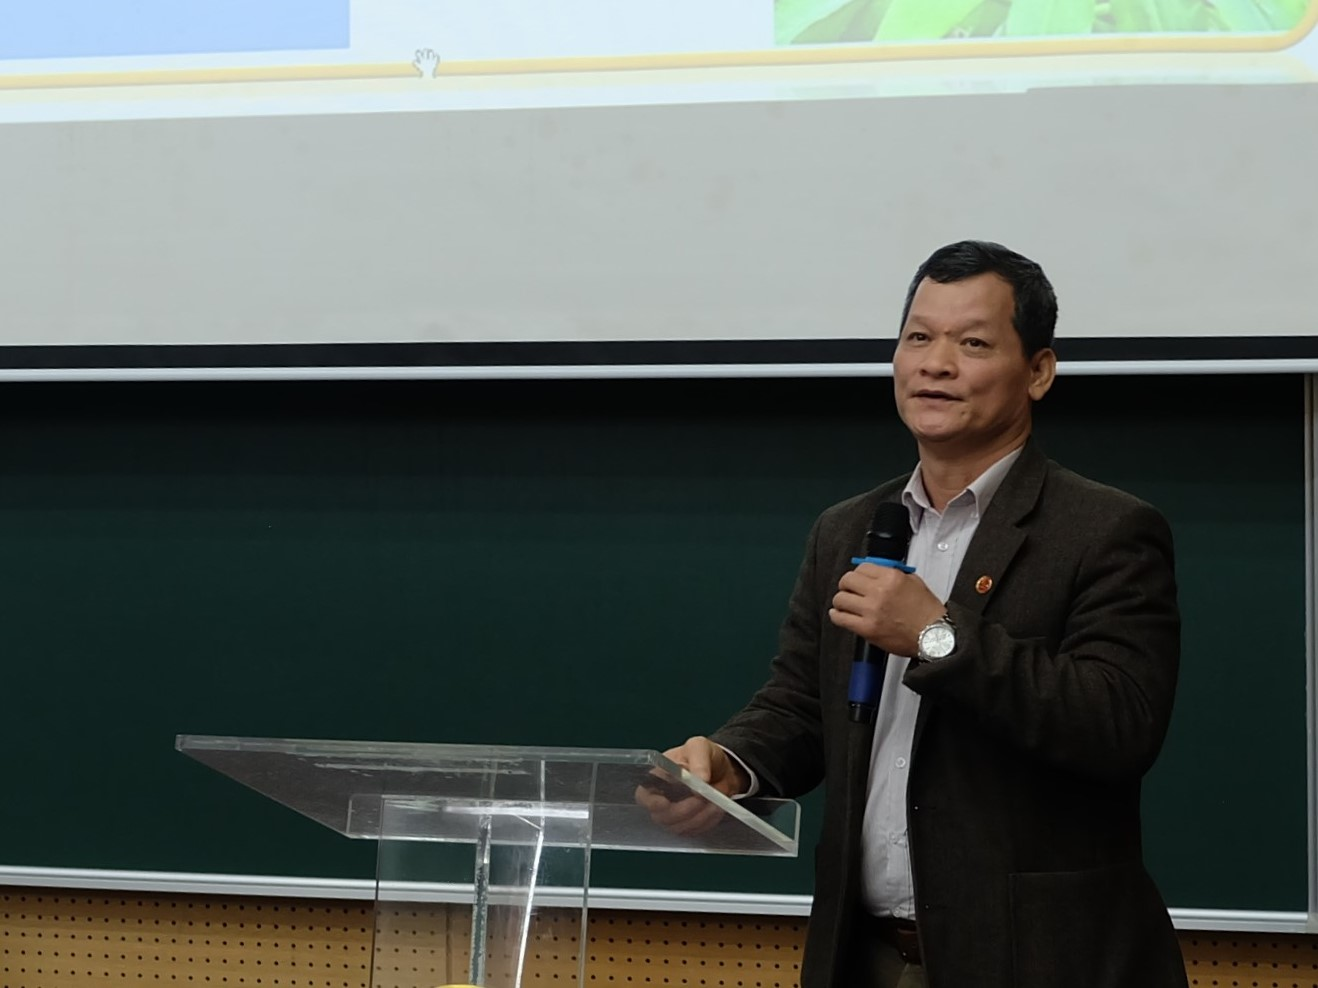
\includegraphics[width= 1\linewidth]{6}
%		\caption{\small\textit{\color{}}}
		\vspace*{-15pt}
	\end{figure}
	$6$. Tích hợp tư duy công dân số trong bài giảng môn Toán, tác giả Nguyễn Thế Minh, Trường Trung học Vinschool Imperia, Hải Phòng; 
	\begin{figure}[H]
		\vspace*{-5pt}
		\centering
		\captionsetup{labelformat= empty, justification=centering}
		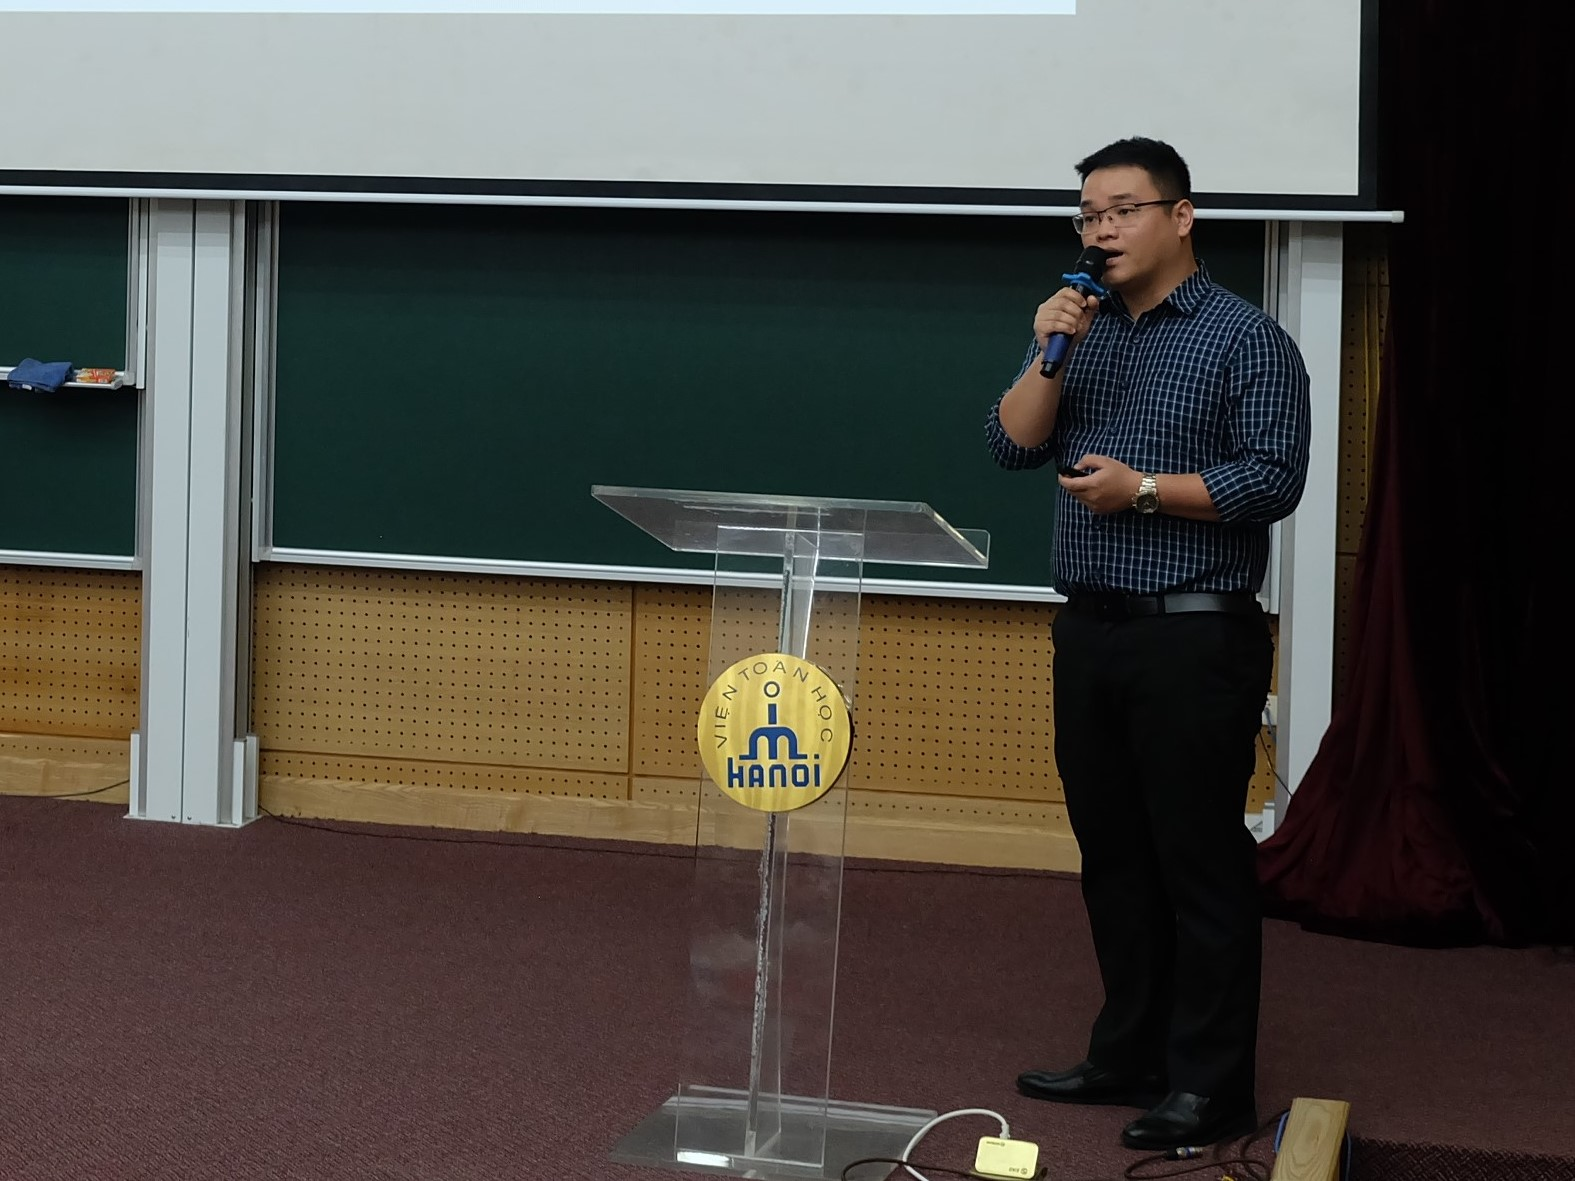
\includegraphics[width= 1\linewidth]{7}
%		\caption{\small\textit{\color{}}}
		\vspace*{-15pt}
	\end{figure}
	$7$. Mập mờ công thức Euler, tác giả Nguyễn Quang Minh, Biên Hoà, Đồng Nai; 
	\begin{figure}[H]
		\vspace*{-5pt}
		\centering
		\captionsetup{labelformat= empty, justification=centering}
		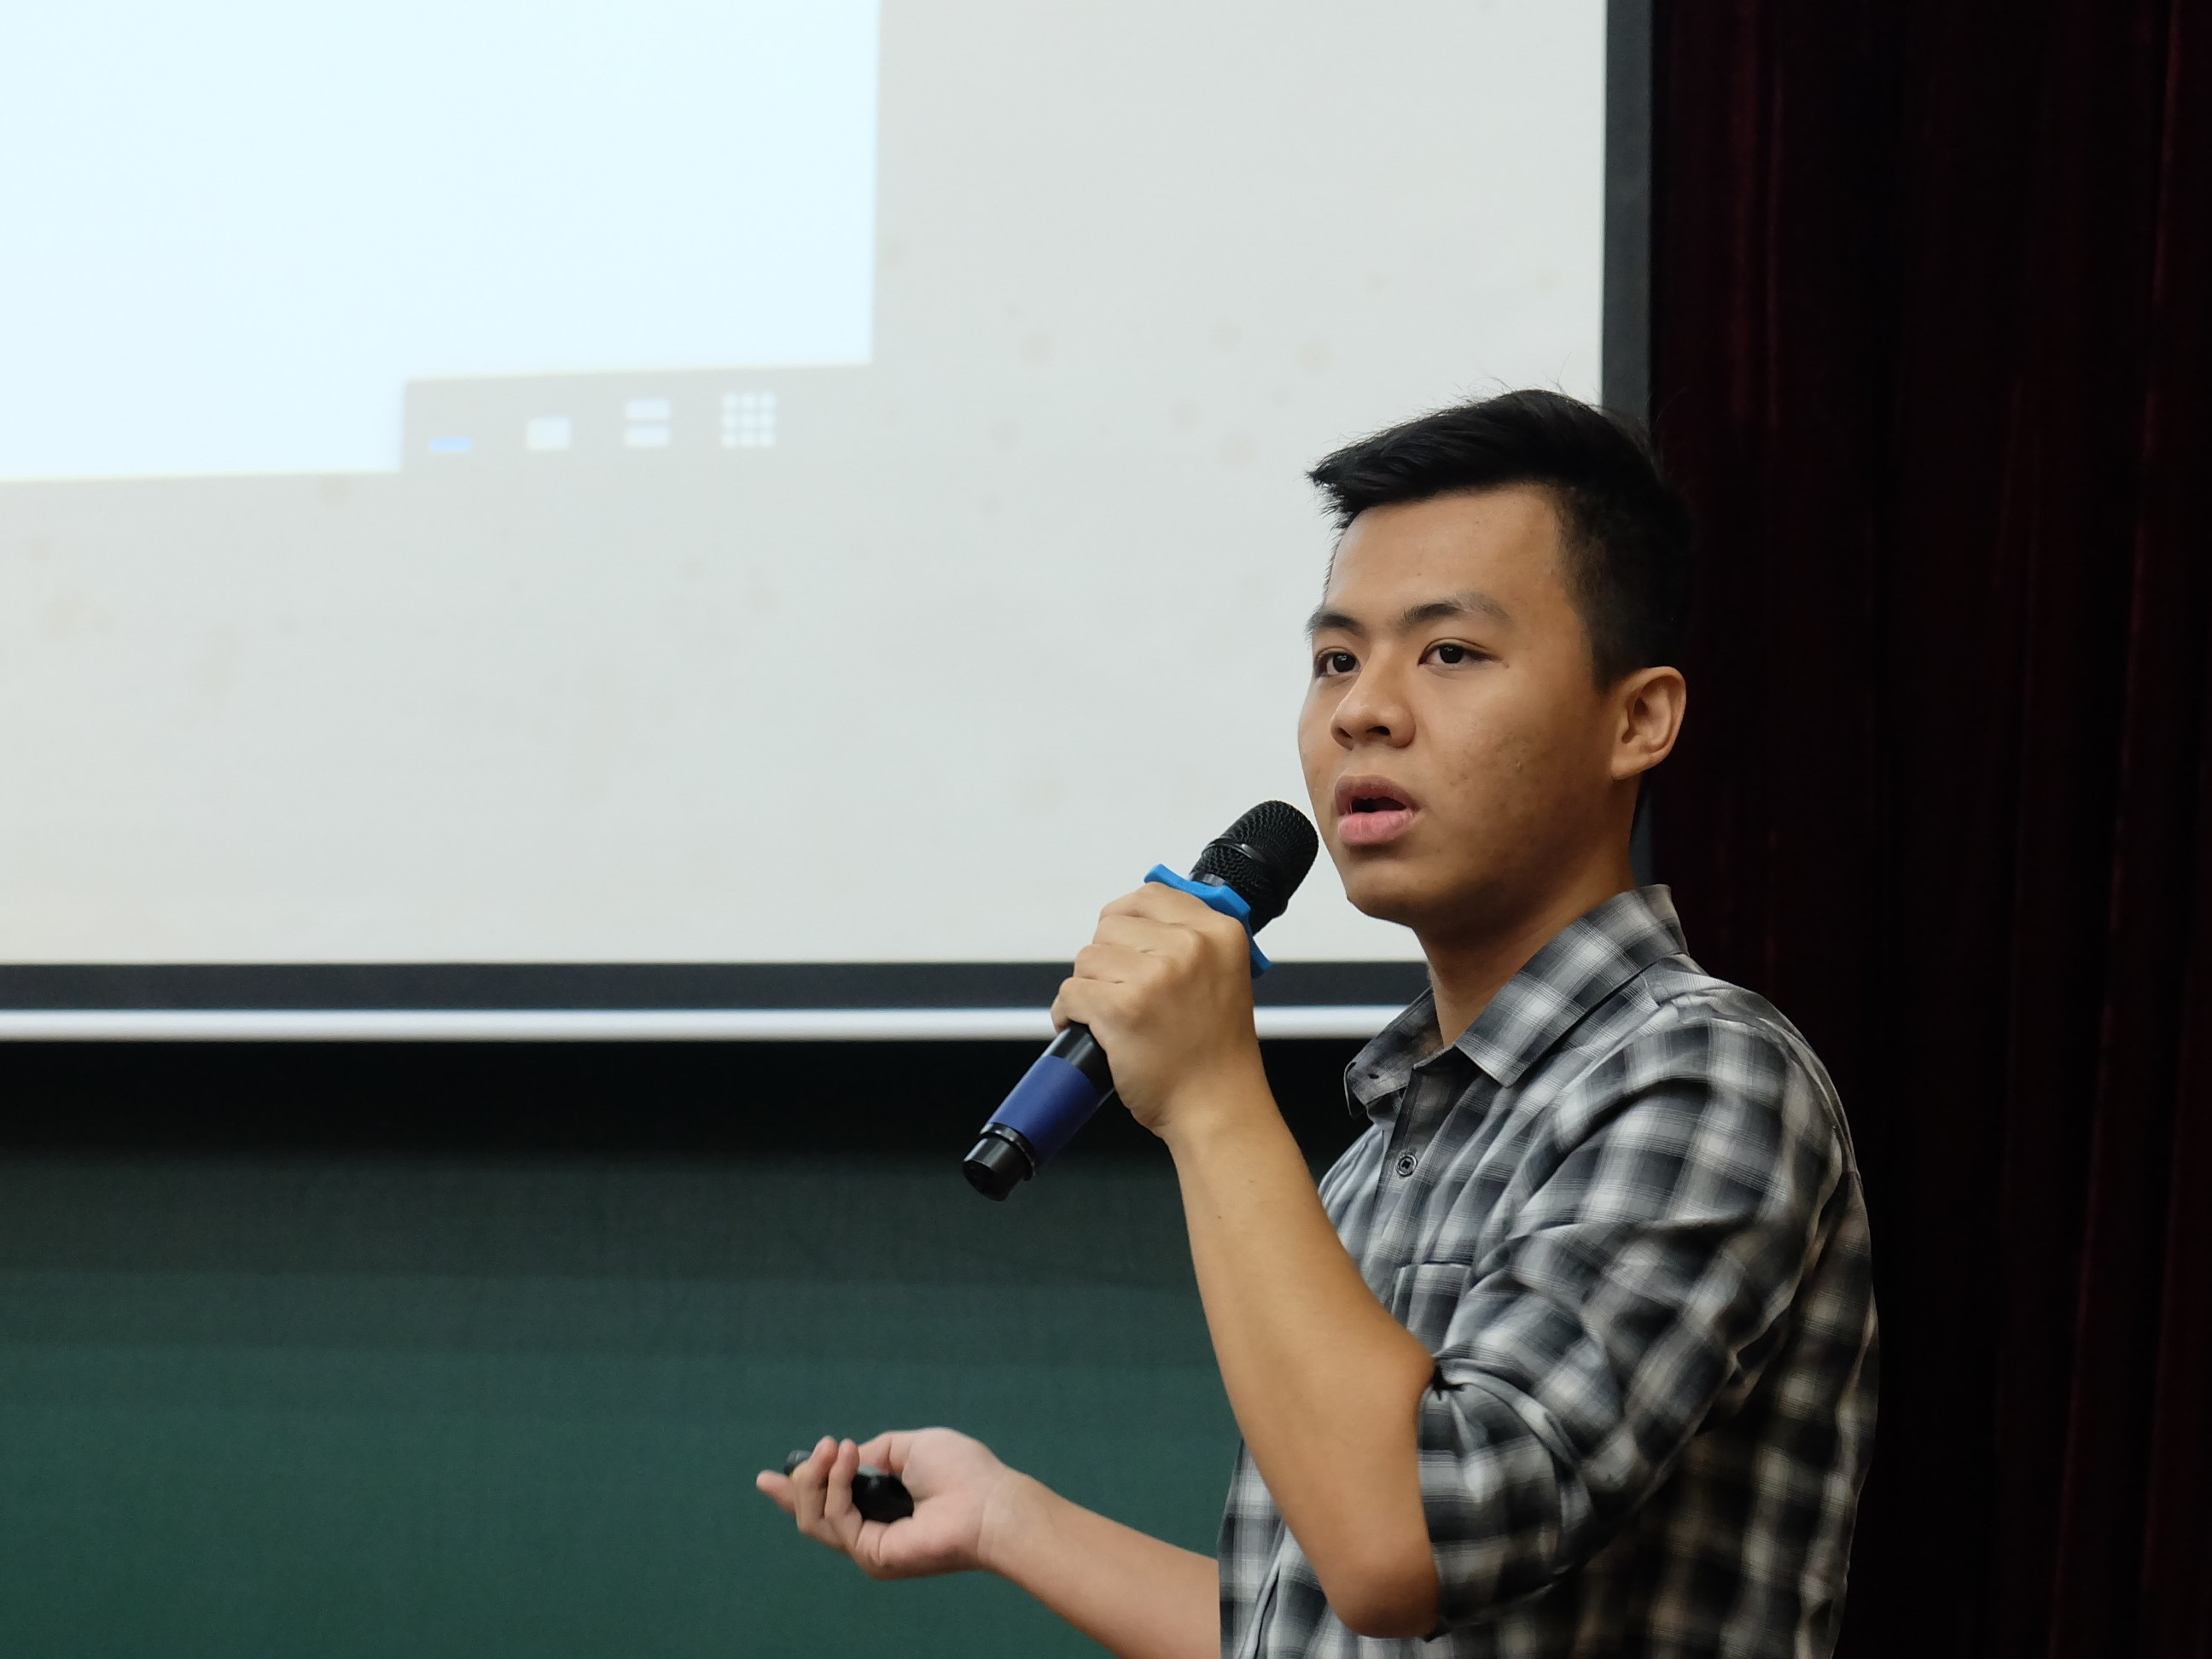
\includegraphics[width= 1\linewidth]{8}
%		\caption{\small\textit{\color{}}}
		\vspace*{-15pt}
	\end{figure}
	$8$. Giải bài toán tập hợp bằng phương pháp ``ô ăn quan", nhóm tác giả Ngô Quốc Trung, Nguyễn Thị Hiền, Trường Liên cấp Hermann Gmeiner Vinh, Nghệ An. 
	\begin{figure}[H]
		\vspace*{-5pt}
		\centering
		\captionsetup{labelformat= empty, justification=centering}
		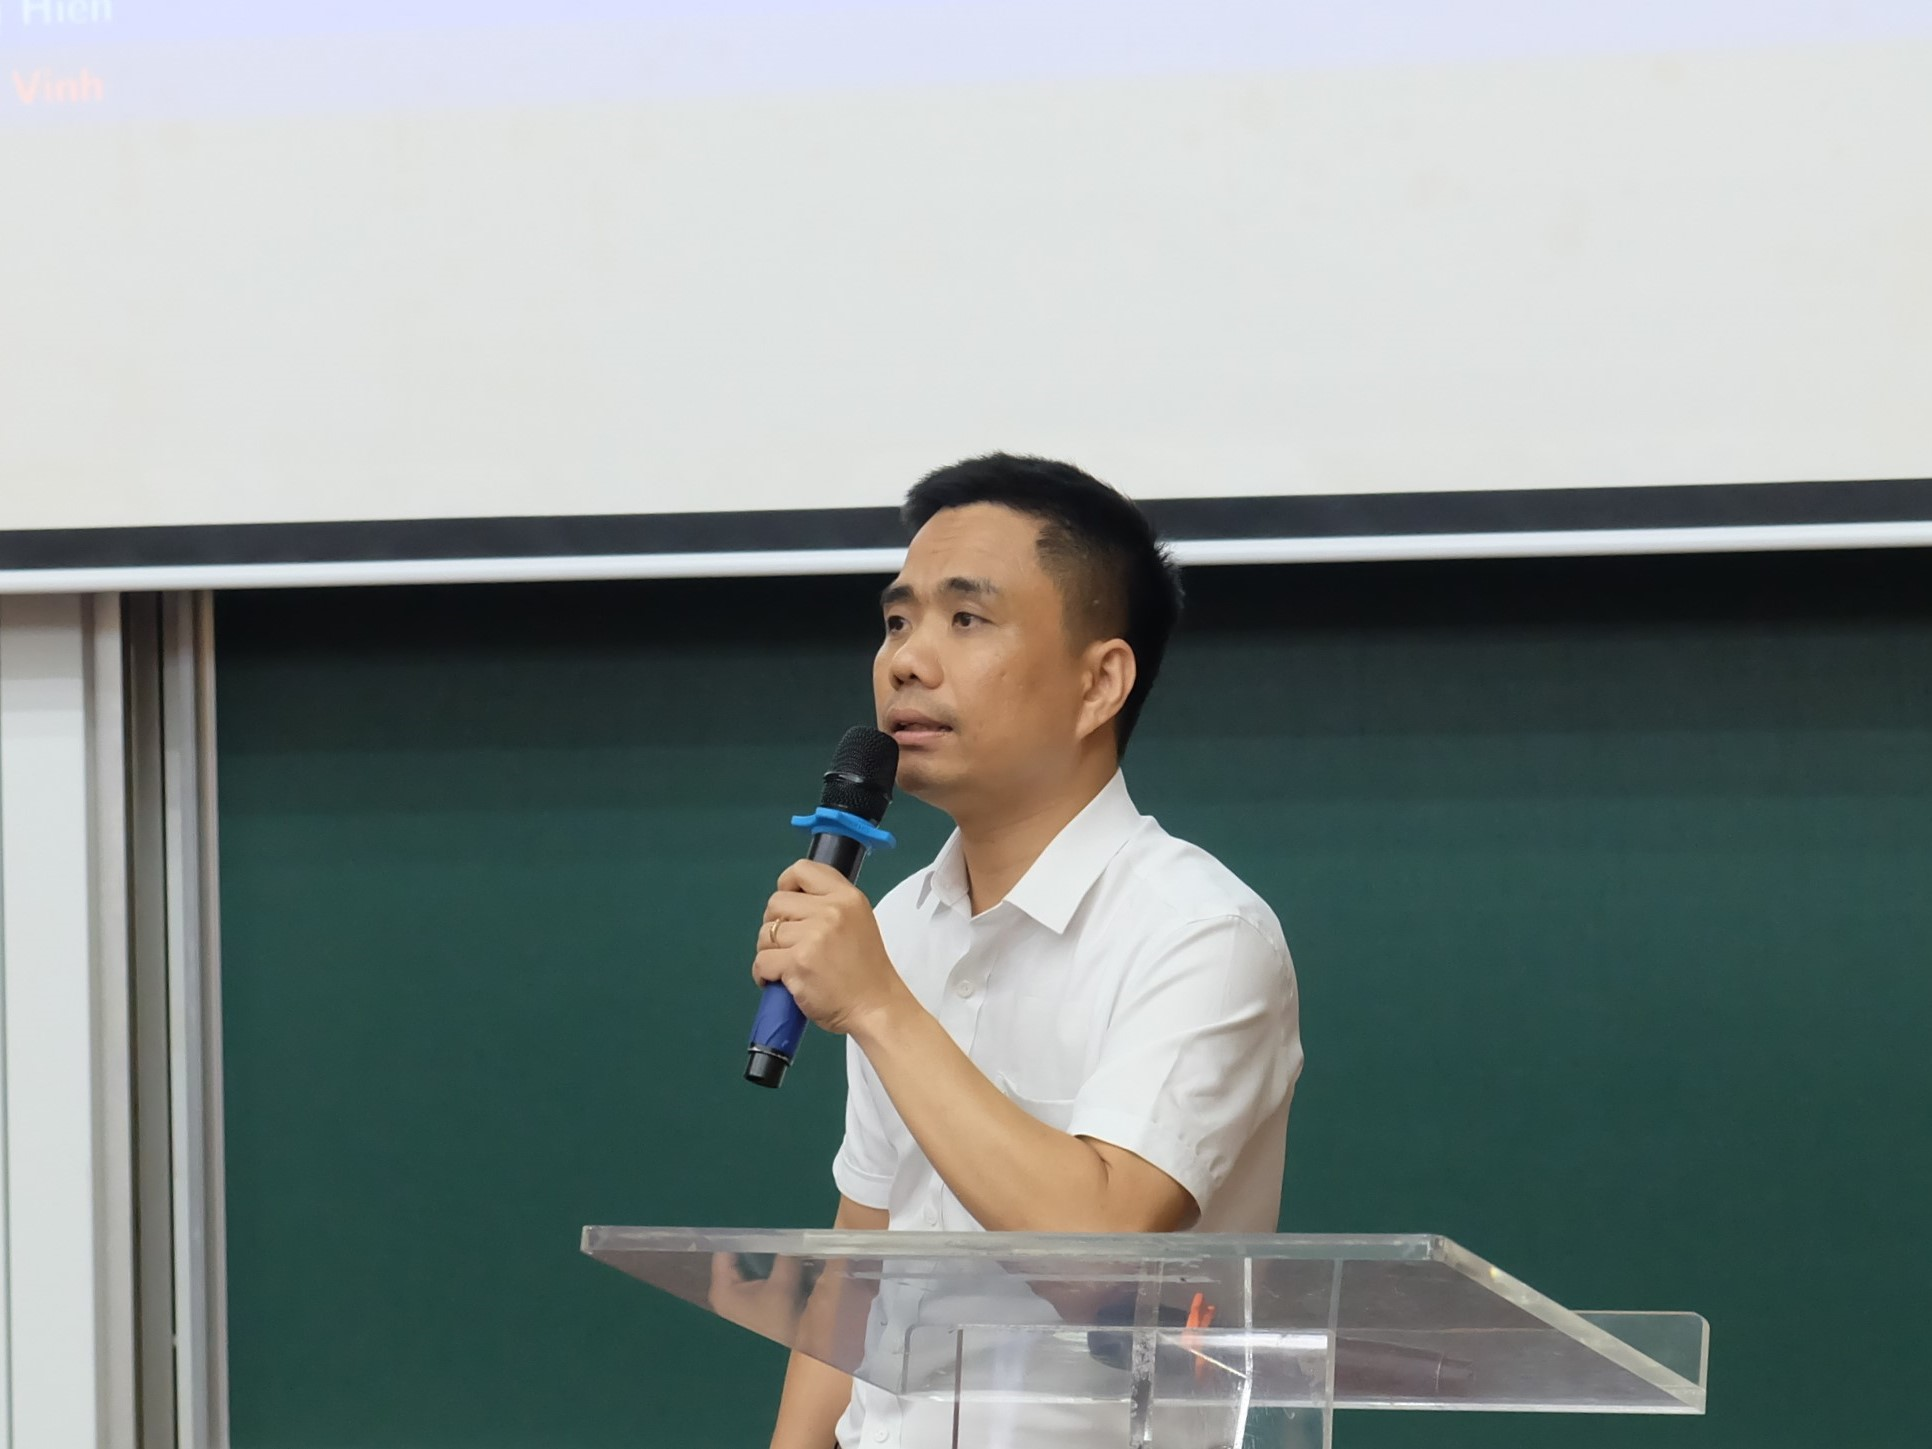
\includegraphics[width= 1\linewidth]{9}
%		\caption{\small\textit{\color{}}}
		\vspace*{-15pt}
	\end{figure}
	Trong khuôn khổ Ngày ``Toán học dành cho mọi người", $8$ nhóm tác giả/tác giả đã thuyết trình các bài giảng và bài viết trước Hội đồng giám khảo. Sau những nhận xét công tâm và đánh giá kỹ lưỡng, Ban Tổ chức đã quyết định trao giải cho các tác giả.
	\vskip 0.1cm
	Về chủ đề ``Tìm hiểu về môn Toán trong ``Chương trình giáo dục phổ thông mới" thông qua một chủ đề cụ thể": Không có giải Nhất, giải Nhì được trao cho bài giảng ``Giải bài toán tập hợp bằng phương pháp ô ăn quan", nhóm tác giả Ngô Quốc Trung, Nguyễn Thị Hiền. Bài viết ``Một cách thiết kế dạy học Toán theo hướng gắn liền với thực tiễn", tác giả Phạm Đức Quang đạt giải Ba. Bài giảng ``Tích hợp tư duy công dân số trong bài giảng môn Toán", tác giả Nguyễn Thế Minh và ``Hình có trục đối xứng", tác giả Nguyễn Thụy Việt Anh đạt giải Khuyến khích. 
	\vskip 0.1cm
	Về các chuyên đề khác, giải Nhất được trao cho bài giảng ``Bổ đề hai đoạn thẳng và một số ứng dụng", tác giả Nguyễn Hữu Tâm. Bài giảng ``Mập mờ công thức Euler", tác giả Nguyễn Quang Minh đạt giải Nhì; ``Lý thuyết đồ thị và một số cấu trúc đáng chú ý", tác giả Hà Trung đạt giải Ba; ``Nét đẹp của phương pháp đếm dưới góc nhìn của số Fibonacci", tác giả Nguyễn Tuấn Anh đạt giải Khuyến khích. 
	\end{multicols}
	\begin{figure}[H]
		\vspace*{5pt}
		\centering
		\captionsetup{labelformat= empty, justification=centering}
		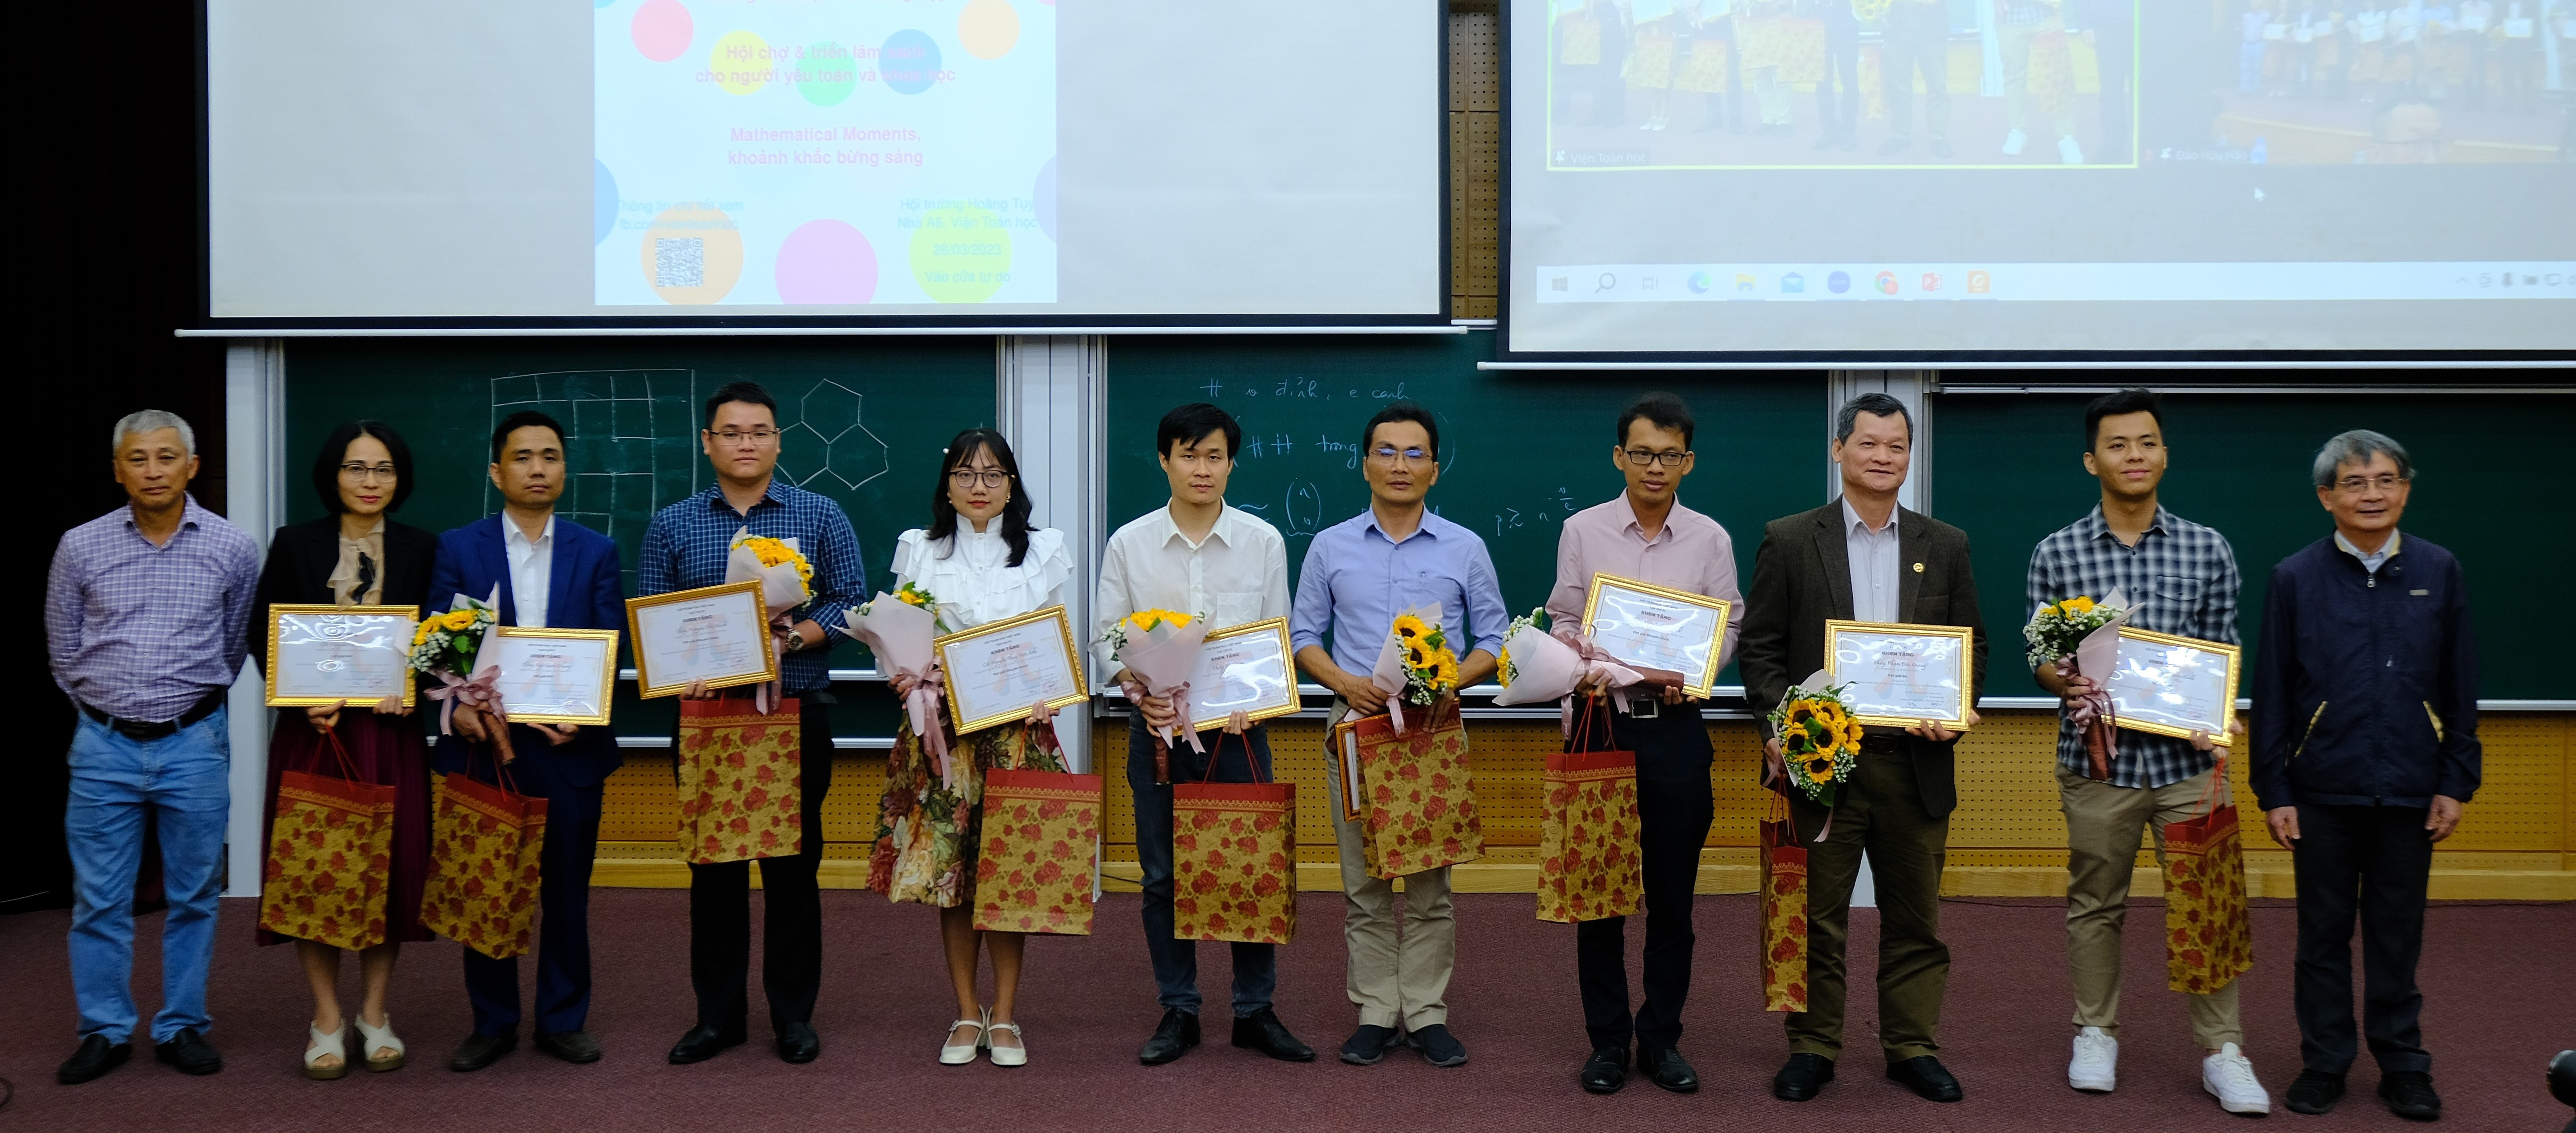
\includegraphics[width= 1\linewidth]{10}
		\caption{\small\textit{\color{doisongtoanhoc}Đại diện ban giám khảo và đại diện gia đình GS Hoàng Tụy trao giải cho các tác giả.}}
		\vspace*{-10pt}
	\end{figure}
	\begin{multicols}{2}
	Theo đánh giá của Ban Tổ chức, chất lượng hồ sơ dự thi của các tác giả tại Kỳ thi ``Bài giảng và bài viết về Toán học, mang tên Hoàng Tụy" lần thứ hai, năm $2023$ cao hơn lần thứ nhất, năm $2021$. Điều đó cho thấy Kỳ thi ``Bài giảng và bài viết về Toán học, mang tên Hoàng Tụy" đã được lan tỏa và hưởng ứng mạnh mẽ, trở thành một nhân tố tích cực góp phần nâng cao chất lượng dạy và học Toán ở cấp trung học phổ thông. 
\end{multicols}